\chapter{Zasady prowadzenia ruchu pociągów}
\section{Ogólne pojęcia}

\textbf{Linia kolejowa} - jest to droga kolejowa mająca początek i koniec wraz z przyległym pasem gruntu, na którą składają się odcinki linii a także budynki, budowle i urządzenia przeznaczone do prowadzenia ruchu kolejowego wraz z zajętymi pod nie gruntami. Punkty początkowe i końcowe linii kolejowych ustala Zarząd PKP PLK S.A.

\textbf{Odcinek} - jest to część linii kolejowej zawarta między sąsiednimi stacjami węzłowymi albo między punktem początkowym lub końcowym linii kolejowej i najbliższą stacją węzłową.

\textbf{Szlak} - jest to część linii kolejowej pomiędzy dwoma posterunkami zapowiadawczymi, lub ostatnim posterunkiem zapowiadawczym i końcowym punktem linii. 

\textbf{Odstęp} - jest to część toru szlakowego pomiędzy posterunkiem zapowiadawczym a posterunkiem odstępowym (semaforem odstępowym), lub bocznicowym, pomiędzy dwoma kolejnymi posterunkami odstępowymi (bocznicowymi), pomiędzy dwoma kolejnymi semaforami odstępowymi blokady wieloodstępowej (samoczynnej) dla tego samego kierunku jazdy przy danym torze.
\footnote{Instrukcja Ir-1}

	\begin{figure}
		\includegraphics[width=0.45\textwidth]{skryptkierownik-img/skryptkierownik-img001.png}
		\caption{Podział sieci kolejowej na odcinki, szlaki i odstępy (wg https://www.bsk.isdr.pl/siec.php)}
		\label{fig:siec}
	\end{figure}


\textbf{Posterunek zapowiadawczy} - jest to posterunek mający możliwość zmiany kolejności jazdy pociągów wyprawianych na tor szlakowy przyległy do tego posterunku. Do posterunków zapowiadawczych należą stacje i posterunki odgałęźne.

\textbf{Granicę} pomiędzy posterunkiem zapowiadawczym a szlakiem stanowi na liniach jednotorowych semafor wjazdowy tego posterunku. Na liniach dwutorowych jest to miejsce znajdowania się semafora wjazdowego i linia prostopadła do osi torów. Jeśli przy danym torze nie ma semafora wjazdowego, jest to miejsce oddalone o 100m od ostatniego rozjazdu lub skrzyżowania torów.

\textbf{Stacja} - jest to posterunek zapowiadawczy, w obrębie którego, oprócz toru głównego zasadniczego, znajduje się co najmniej jeden tor główny dodatkowy, a pociągi mogą rozpoczynać i kończyć jazdę, krzyżować się i wyprzedzać, jak również zmieniać skład lub kierunek jazdy. Duże stacje mogą być podzielone na rejony stanowiące osobne posterunki zapowiadawcze. Stacja, na której układ torów umożliwia jedynie krzyżowanie i wyprzedzanie pociągów, nazywa się mijanką.

\textbf{Pociąg} - jest to skład wagonów lub innych pojazdów kolejowych sprzęgniętych z czynnym pojazdem trakcyjnym albo pojazd trakcyjny – osygnalizowany i przygotowany do jazdy lub znajdujący się w drodze.

Na stacjach tory kolejowe dzielą się na tory: główne, specjalnego przeznaczenia i boczne.

Tory przystosowane do jazd pociągowych nazywają się \textbf{torami głównymi}. Dzielą się one na tory główne zasadnicze i tory główne dodatkowe. Tory główne będące przedłużeniem torów szlakowych nazywają się torami głównymi \textbf{zasadniczymi}, natomiast pozostałe tory główne torami głównymi \textbf{dodatkowymi}. Do torów specjalnego przeznaczenia należą: żeberka ochronne, tory dojazdowe do bocznic, komunikacyjne, wyciągowe, bocznicowe. Inne tory na stacjach są torami bocznymi.

Tory na szlakach i stacjach określa się liczbami. Na \textbf{szlaku} korzysta się z liczebników głównych (tor nr jeden, tor nr dwa), zaś w stacji liczebnikami porządkowymi (pierwszy, drugi). Numeracja torów na szlakach dwutorowych definiowana jest patrząc od początku linii (km 0,0) ku jej końcowi, gdzie tor prawy jest torem nr 1, zaś tor lewy torem
nr 2.
	\begin{figure}
	\includegraphics[width=0.45\textwidth]{skryptkierownik-img/tory-numery.png}
	\caption{Rodzaje torów stacyjnych i ich numeracja (wg https://www.bsk.isdr.pl/siec.php)}
	\label{fig:numeracja-torow}
\end{figure}

Na \textbf{stacjach} torem nr 1 (pierwszym) jest tor główny zasadniczy będący przedłużeniem toru szlakowego nr 1. Na stacjach węzłowych miarodajną jest linia kolejowa wyższej kategorii, a przy równorzędności linii przyjmuje się linię o większym obciążeniu ruchem pociągów. Kolejne tory stacyjne po \textbf{prawej stronie} toru głównego zasadniczego patrząc od początku linii określa się kolejnymi liczbami \textbf{nieparzystymi}, a znajdujące się po \textbf{lewej} stronie toru głównego zasadniczego kolejnymi liczbami \textbf{parzystymi}. Jeśli tory stacyjne podzielone są na grupy, w sposób ustalony w regulaminie technicznym, dla każdej grupy ustala się osobną dziesiątkę lub setkę liczb.

Przy prowadzeniu ruchu pociągów w ustalonych sytuacjach stosuje się \textbf{telefoniczne zapowiadanie pociągów}, które polega na porozumiewaniu się dyżurnych ruchu za pośrednictwem kablowej łączności telefonicznej. Telefoniczne zapowiadanie pociągów stosuje się zawsze na liniach nie wyposażonych w urządzenia blokady liniowej lub na na liniach kolejowych z blokada liniową w przypadkach, gdy nie jest lub nie może ona być podstawą prowadzenia ruchu. Podstawą prowadzenia pociągu jest między innymi przekazywanie numeru pociągu wyprawianego do kolejnego posterunku następczego. Jeżeli nie wykonują tego urządzenia SRK to stosuje się telefoniczne zapowiadanie pociągów w określonym zakresie dla poszczególnych typów szlaków i urządzeń SRK. 
Na sieci PKP nie ma urządzeń SRK automatycznie przekazujących numer pociągu w związku z czym łączność telefoniczna przy prowadzeniu ruchu pociągów jest stosowana na całej sieci kolejowej.

\section{Budowa toru i rozjazdu}

Nawierzchnia kolejowa oznacza drogę dla pojazdów szynowych. Jest to konstrukcja, składająca się z toru kolejowego lub rozjazdu, po którym poruszają się pojazdy szynowe, elementów podporowych (podkłady lub podrozjazdnice), elementów przytwierdzających i łączących (m.in. złączek) oraz podsypki. Tak jak w przypadku konstrukcji budowlanej, podstawowym zadaniem nawierzchni kolejowej jest przeniesienie obciążenia eksploatacyjnego na podtorze.
Tor kolejowy to dwa toki szynowe ułożone w ustalonej odległości od siebie stanowiące podstawowy układ nośny nawierzchni kolejowej, której układ geometryczny przystosowany jest do bezpiecznego ruchu pojazdów kolejowych, z prędkościami oraz naciskami określonymi poprzez parametry techniczno-eksploatacyjne. Parametry techniczno - eksploatacyjne dla linii kolejowej ustala zarządca infrastruktury, czyli podmiot wykonujący działalność polegającą na zarządzaniu infrastrukturą kolejową na zasadach określonych w ustawie o transporcie kolejowym.
Ze względu na rodzaj konstrukcji nawierzchni, wyróżniamy nawierzchnie podsypkowe (najczęściej stosowane) oraz bezpodsypkowe (stosowane zazwyczaj w tunelach oraz na mostach i wiaduktach). 

\begin{figure}
	\includegraphics[width=0.45\textwidth]{skryptkierownik-img/budowa-toru.png}
	\caption{Elementy nawierzchni kolejowej: 1 - szyny, 2 - podkłady, 3 - podsypka,źródło: Drogi Szynowe, Gdańsk 2013}
	\label{fig:tory}
\end{figure}

Nawierzchnia kolejowa składa się z:
\begin{itemize}
\item szyn,
\item systemu przytwierdzeń szyn do podkładów,
\item łączy szynowych i złączek,
\item podkładów,
\item podsypki 
\end{itemize}


Zasadniczą częścią konstrukcji toru kolejowego są szyny. Zadaniem szyn jest przejęcie sił pionowych i poprzecznych z kół taboru i przeniesienie ich na podkłady. Szyny są elementem prowadzącym zestawy kołowe, nadając im właściwy kierunek jazdy. Dodatkowo szyny przewodzą prąd zasilający pojazdy trakcyjne na liniach zelektryfikowanych, są również elementem systemu urządzeń sterowania ruchem kolejowym (odcinki izolowane). W Polsce zasadniczo stosuje się trzy typy szyn kolejowych oznaczonych symbolami S42, S49 (49E1)
oraz UIC60 (60E1).

Tor kolejowy może być wykonany jako klasyczny lub bezstykowy. Tor klasyczny stanowi konstrukcję, w której szyny o normatywnej długości są ze sobą połączone na stałe za pomocą złączek i przytwierdzone do podkładów. Szyny w torze klasycznym połączone są za pomocą złącz:
podpartych na podzłączowych podwójnych podkładach drewnianych z połączeniem szyn łubkami i czterema śrubami łubkowymi;
wiszących z połączeniem szyn łubkami wzmocnionymi i sześcioma śrubami łubkowymi 

Tor bezstykowy stanowi konstrukcję, w której kolejne szyny łączone są ze sobą trwale przy pomocy zgrzewania elektrooporowego, spawania termitowego lub łukowego. Długość odcinka toru bezstykowego jest nieograniczona. Odcinki toru z szynami spawanymi lub zgrzewanymi o długości większej niż 180 m uważa się za tor bezstykowy. Do budowy toru bezstykowego w torach na szlakach i głównych zasadniczych stosuje się szyny długie zgrzewane stacjonarnie. Łączenie szyn długich oraz szyn w pozostałych torach powinna być wykonana metodą zgrzewania, spawania termitowego lub inną metodą dopuszczoną do stosowania przez zarządcę infrastruktury. 

Rozjazd kolejowy to specjalna konstrukcja wielotorowa wykonana z szyn kolejowych, kształtowników stalowych oraz innych elementów, która umożliwia przejazd pojazdów kolejowych z jednego toru na drugi z określoną prędkością.
Rozjazd zwyczajny składa się z trzech podstawowych zespołów/bloków, tj.:
A – zwrotnicy, służącej do kierowania zestawów kołowych pojazdu kolejowego
z jednego toru na drugi tor,
B – szyn łączących,
C – krzyżownicy z kierownicami i szynami tocznymi, stanowiącej przecięcie szyn dwóch torów (w tym dziób krzyżownicy i szyny skrzydełkowe)

\begin{figure}
	\includegraphics[width=0.45\textwidth]{skryptkierownik-img/rozjazd.png}
	\caption{Elementy rozjazdu, źródło: Krzysztof Zajaczkowski - pl.wikipedia.org: ''Plik:Bud\_rozjazdu.jpg'', GFDL}
	\label{fig:rozjazd}
\end{figure}
Zwrotnica rozjazdu to jego część, zawierająca elementy ruchome, umożliwiająca przejazd pojazdu kolejowego z jednego toru na drugi przy zachowaniu ciągłości toków szynowych.
Zwrotnica w rozjeździe zwyczajnym składa się z: opornicy prostej, iglicy łukowej, iglicy prostej, opornicy łukowej.
W celu umożliwienia przestawiania zwrotnic, a jednocześnie dla zapewnienia prawidłowego przylegania iglicy do opornicy i niedopuszczenia do samoczynnego odsunięcia się iglicy od opornicy pod przejeżdżającym taborem, stosuje się zamknięcia nastawcze.
Wyróżnia się następujące zamknięcia nastawcze:
\begin{itemize}
	\item hakowe,
	\item suwakowe,
	\item specjalne – pozostałe rodzaje zamknięć nastawczych, różniące się od standardu
	konstrukcyjnego ww. zamknięć nastawczych, np. VCC, HRS, Spherolock, Hydrostar.
\end{itemize}

Zamknięcie nastawcze hakowe znajduje się przy początku iglic i umieszczone jest zazwyczaj między 2 i 3 podrozjazdnicą.
Zamknięcie hakowe jest rozpruwalne, to znaczy, że przy jeździe po zwrotnicy nastawionej do innej jazdy, zwrotnica może być przestawiona przez koła pojazdu podczas ruchu w kierunku zbieżnym (od krzyżownicy ku zwrotnicy) bez uszkodzenia konstrukcji zamknięcia nastawczego.

Jeżeli należy zabezpieczyć rozjazd przed przypadkowym przełożeniem (np. w trakcie awarii), można wykorzystać zamek trzpieniowy - do zabezpieczenia iglicy odlegającej, lub sponę iglicową do zabezpieczenia iglicy przylegającej. Miejsce montażu zamka lub spony jest pomalowane na bocznej ścianie szyny na biało.

W sytuacji rozprucia rozjazdu (wjazd na niepoprawnie ułożony rozjazd od strony krzyżownicy) zabronione jest cofanie składu bo doprowadzi to do wykolejenia. Jeśli konieczne jest ruszenie składem, dopuszczalne to jest wyłącznie do przodu i wyłącznie w sytuacji zagrożenia życia.

Krzyżownica umożliwia swobodny przejazd w jednym poziomie kół pojazdu kolejowego przez miejsce krzyżowania się szyn.
Zespół krzyżownic w rozjeździe zwyczajnym składa się z:
krzyżownicy zwyczajnej, dwóch kierownic, dwóch szyn łączących.
Krzyżownica zwyczajna składa się z dziobnicy, dwóch szyn skrzydłowych i dwóch szyn tocznych z kierownicami. Wewnętrzne toki szynowe przecinających się torów w krzyżownicy tworzą
dziobnicę, która składa się z dzioba i szyn dziobowych. Dziób krzyżownicy jest to środkowy element
krzyżownicy tworzący przednią część dziobnicy. Kierownica wraz z szyną toczną oraz elementami
mocującymi tworzy tzw. urządzenie kierownicy.

Szyny o specjalnym profilu wraz z szynami tocznymi, ułożone naprzeciw dzioba krzyżownicy, tworzą kierownicę.
Służy ona do bezpiecznego przeprowadzenia zestawu kołowego przez obszar krzyżownicy, w którym występuje nieciągłość toków szynowych.  Zestaw kołowy, przechodząc przez krzyżownicę, ociera się wewnętrzną
powierzchnią obrzeża o boczną powierzchnię kierownicy i dzięki temu nastawia obrzeże drugiego koła zestawu kołowego we właściwym kierunku. Dzięki temu krzyżownice zwyczajne nie mają odcinków pozbawionych prowadzenia zestawów kołowych.

Jeżeli rozjazd jest ustawiany ręcznie, to przeciwwaga jest pomalowana na dwa kolory, czarny i biały, oznaczające położenie kierunku jazdy. Kolor biały oznacza kierunek zasadniczy (+). Jeżeli na przeciwwadze w części białej znajdują się dwa czerwone paski, to dozwolona jest obsługa rozjazdu przez drużynę manewrową.

Istnieje możliwość sterowania pracą rozjazdu w sposób mechaniczny z wykorzystaniem dźwigni nastawczych, naprężaczy i drutów pędniowych, lub elektryczny (silnik).

(więcej ilustracji https://utk.gov.pl/download/1/41355/Poradnikdlakomisjikolejowych-toryrozjazdyiskrzyzowaniatorow.pdf)

\section{Przygotowanie pociągu do drogi}

Przed wyprawieniem pociągu w drogę, należy go przygotować do jazdy. W zakres przygotowania wchodzą następujące czynności:

\begin{enumerate}
\item zestawienie zgodne z parametrami określonymi w wewnętrznym rozkładzie jazdy pociągów,
\item wykonanie oględzin technicznych, o ile są wymagane
\item wykonanie wymaganej próby hamulca
\item osygnalizowanie pociągu
\item sprawdzenie czy nie ma przeszkód pod kołami pociągu (dotyczy płozów hamulcowych, czy nie zamknięto wykolejnicy,
etc.) i czy jego hamulce ręczne oraz postojowe są odhamowane
\item posiadanie dokumentów określonych odrębnymi przepisami, które powinny się znajdować w pojeździe kolejowym (wg. przepisów wew. KŚL są to książka pojazdu z napędem, karta próby hamulca, które powinny się znajdować w czynnej kabinie maszynisty, oraz wykaz pojazdów kolejowych w składzie pociągu - u kierownika pociągu)
\end{enumerate}
Po przygotowaniu pociągu do drogi i jego poprawnym osygnalizowaniu należy zgłosić gotowość pociągu do odjazdu. Zgłoszenia dyżurnemu ruchu dokonuje wskazany w regulaminie technicznym pracownik przewoźnika (maszynista lub kierownik pociągu) podając numer pociągu, numer i serię pojazdu trakcyjnego, długość pociągu w metrach, masę ogólną pociągu, informację o TWR, towarach niebezpiecznych lub przesyłkach nadzwyczajnych, oraz podając numer zgody, godzinę zgłoszenia i nazwisko zgłaszającego. Przed odjazdem pociągu dyżurny ruchu powinien przekazać obsadzie pociągu informacje, polecenia i zezwolenia (rozkazy pisemne).

\chapter{Regulaminy techniczne posterunków i odcinków zdalnego prowadzenia ruchu}

Regulamin techniczny stacji i posterunku składa się z tzw. działek które opisują:
\begin{itemize}
	\item położenie posterunku ruchu na linii (wraz z opisem typu blokady liniowej)
	\item sposób prowadzenia ruchu na przyległych szlakach (przy pomocy blokady liniowej lub telefonicznego zapowiadania)
	\item wykaz posterunków technicznych (nastawczych, zwrotniczowskich) na stacji z opisem rodzaju urządzeń oraz granic okręgów nastawczych
	\item skrajnie budowli na przyległych szlakach
	\item przejazdy i przejścia na przyległych szlakach z opisem kategorii, oraz dodatkowymi zaleceniami
	\item wykaz torów stacyjnych, z ich numeracją, opisem przeznaczenia, długością użyteczną, możliwością przejazdu przekroczonej skrajni.
	\item wykaz rozjazdów z opisem położenia zasadniczego, sposobu nastawiania
	\item przyjmowanie i wyprawianie pociągów z towarami niebezpiecznymi, TWR i przesyłkami nadzwyczajnymi oraz sposób postępowania przy sytuacjach awaryjnych
	\item opis przebiegów pociągowych i manewrowych dla wjazdu i wyjazdów
	\item środki pomocnicze dla zabezpieczania w przypadku ''Sz'' lub innych sytuacji nietypowej
	\item sposób zabezpieczania przed zbiegnięciem pojazdów odstawionych na postój (\textbf{dz.40})
	\item sposób zgłoszenia gotowości do odjazdu pociągu
	\item regulaminy bocznic, sposoby prowadzenia jazd trakcyjnych, etc.
	\item plan schematyczny posterunku
\end{itemize}
	\begin{figure}
	\includegraphics[width=0.45\textwidth]{skryptkierownik-img/komory_sygnalowe_pl.png}
	\caption{Symbole komór sygnałowych, od lewej czerwona, zielona, pomarańczowa, niebieska, matowobiała}
\end{figure}

Na planach schematycznych posterunków ruchu używa się znormalizowanych symboli oznaczających cechy urządzeń SRK oraz podawanych sygnałów na sygnalizatorach.

\chapter{Rodzaje urządzeń sterowania ruchem kolejowym i łączności}

Blokada stacyjna uzależnia nastawnie tego samego posterunku ruchu, czyli na przykład w obrębie stacji, a blokada liniowa są to urządzenia techniczne przeznaczone do regulacji następstwa pociągów oraz ustalenia kierunku ruchu na szlaku (uzależnienie czynności nastawni sąsiednich posterunków ruchu). 

\textbf{Półsamoczynne blokady liniowe} uniemożliwiają wyprawienie pociągu na szlak (odstęp) do czasu potwierdzenia przybycia w całości poprzedniego pociągu do następnego posterunku ruchu. Z reguły potwierdzenie to dawane jest przez personel ruchu, po wzrokowym stwierdzeniu, że pociąg wjechał z sygnałami końca pociągu, a sygnały zezwalające na semaforach podawane są ręcznie. Konieczność obsady posterunków odstępowych powodowała, że szlaki z półsamoczynną blokadą liniową rzadko dzielono na odstępy.

Na szlakach z półsamoczynną blokadą liniową ruch pociągów regulowany jest w oparciu o blokowanie i zwalnianie blokady. Sygnał zezwalający na wyjazd na szlak (odstęp) może być podany tylko jeden raz do czasu zwolnienia blokady. Zmiany stanu blokady są jednocześnie informacją dla personelu o wyprawieniu lub przyjęciu pociągu przez sąsiedni posterunek ruchu.

\textbf{Samoczynne blokady liniowe} wyposażone są w układową kontrolę niezajętości odstępów, a sygnały na semaforach odstępowych wyświetlane są samoczynnie, w zależności od sytuacji ruchowej. Odstępy samoczynnej blokady liniowej są krótkie, co pozwala na uzyskanie dużej przepustowości.

Przy samoczynnej blokadzie liniowej ruch pociągów regulowany jest na podstawie kontroli niezajętości odstępów blokowych przez obwody torowe lub liczniki osi. Na szlaku stosowane są samoczynne semafory odstępowe, na których sygnały wyświetlane są samoczynnie, zależnie od sytuacji ruchowej i ustawionego kierunku ruchu. Prowadzenie ruchu pociągów, poza zmianą kierunku ruchu, nie wymaga obsługi urządzeń blokady.

Na szlaku jednotorowym dwukierunkowym wyposażonym w SBL, jak na każdym szlaku jednotorowym, jest ustalony jeden kierunek ruchu, jako uprzywilejowany. Najczęściej jest to kierunek zgodny ze wzrastającym kilometrowaniem na linii. Według tego kierunku jest ustalony stan zasadniczy blokady liniowej (każdego typu). 
Jeżeli SBL znajduje się w stanie zasadniczym (szlak jest wolny) to świecą się semafory kierunku uprzywilejowanego, natomiast dla kierunku przeciwnego semafory są wygaszone, z wyjątkiem ostatniego semafora SBL ze wskaźnikami W18, który zawsze jest oświetlony. 
Przełączenie kierunku ruchu następuje po telefonicznym porozumieniu dyżurnych ruchu sąsiednich posterunków ruchu i po obsłużeniu odpowiednich manipulatorów blokady (żądania pozwolenia, dania pozwolenia) według ustalonych zasad obsługi tych urządzeń - sytuacja podobna do tej z PBL. 

Blokady liniowe \textbf{jednokierunkowe} przeznaczone są dla szlaków dwutorowych i ich działanie ogranicza się do regulacji następstwa ruchu pociągów w jednym kierunku. Przebiegi na tory szlakowe w kierunku przeciwnym do zasadniczego nie są przewidziane lub są nieuzależnione od stanu blokady liniowej.

Blokady liniowe \textbf{dwukierunkowe} umożliwiają prowadzenie ruchu pociągów po torze szlakowym w obu kierunkach. Ustawienie wybranego kierunku ruchu wymaga przeważnie dania pozwolenia przez personel posterunku zapowiadawczego mającego przyjąć pociąg. W przypadku obsługi blokady liniowej przez nastawnię wykonawczą, danie pozwolenia powinno być uzależnione od otrzymania polecenia od dyżurnego ruchu, przekazanego przez urządzenia (otrzymanie zlecenia). W niektórych typach blokad liniowych dwukierunkowych, poza stanem ustawionego kierunku ruchu występować może stan neutralny, w którym żaden z kierunków nie jest włączony.

 


\chapter{Sygnalizacja kolejowa}

\section{Wskaźniki}

\begin{center}
	\begin{figure}
		\includegraphics[width=0.5\textwidth]{skryptkierownik-img/skryptkierownik-img003.png}
		\caption{Wskaźniki przytorowe (wg http://pkprepo.net/wskazniki-kolejowe-pkp/)}
		\label{fig:wskazniki}
	\end{figure}
\end{center}

\subsection{W1 - wskaźnik usytuowania}

Prostokątna biała tablica z czarnym obramowaniem, a na niej dwa czarne kąty, oparte na krótszych bokach prostokąta, jeden nad drugim, stykające się wierzchołkami w środku tablicy. Wskaźnik W 1 oznacza miejsce ustawienia tarczy ostrzegawczej semaforowej lub przejazdowej, a na szlakach z samoczynną blokadą liniową czterostawną - przedostatniego
semafora odstępowego blokady samoczynnej na szlaku przed semaforem wjazdowym. Wskaźnik W1 stawiany jest bezpośrednio przed tarczą ostrzegawczą kształtową lub świetlną. Informuje, że TO podaje sygnał, jakiego należy spodziewać się na semaforze, do którego się ona odnosi. Dlatego też wskaźnika W1 nie stawia się przed TO nieruchomą.

	\begin{figure}
		\includegraphics[width=0.45\textwidth]{skryptkierownik-img/skryptkierownik-img004.jpg}
		\caption{Wskaźnik W1}
	\end{figure}

\subsection{W3 - wskaźnik unieważnienia + W15 wskaźnik zmiany lokalizacji}

Wskaźnik W 3 {\textquotedbl}Wskaźnik unieważnienia{\textquotedbl} oznacza, że znajdujący się z prawej strony toru przy
tym wskaźniku semafor lub tarcza zatrzymania nie odnoszą się do toru, przy którym stoi wskaźnik. Wskaźnik W 3 ustawia
się z prawej strony toru przy znajdującym się tam semaforze lub tarczy zaporowej dla oznaczenia, że semafor ten lub
tarcza zaporowej nie odnoszą się do toru, przy którym stoi wskaźnik. Sygnał dzienny stanowi słup semafora pomalowany na
szaro, zaś sygnał nocny białe światło świecące ciągle na szczycie.

Wskaźnik W 15 {\textquotedbl}Wskaźnik zmiany lokalizacji{\textquotedbl} oznacza, że semafor, sygnalizator powtarzający lub tarcza ostrzegawcza nie są umieszczone w miejscu, w którym powinny się znajdować, pomimo to odnoszą się do toru, przy którym stoi wskaźnik. Kwadratowa biała tablica z czarnym trójkątem zwróconym ostrzem w kierunku semafora,
sygnalizatora powtarzającego lub tarczy ostrzegawczej (trójkąt równoramienny, którego podstawą jest bok kwadratu, a
wierzchołek skierowany do sygnalizatora leży na środku przeciwległego boku). Wskaźnik W 15 ustawia się w tym miejscu, w
którym powinny być ustawione: semafor, sygnalizator powtarzający lub tarcza ostrzegawcza.

	\begin{figure}
		\includegraphics[width=0.45\textwidth]{skryptkierownik-img/wskaznik-w3.jpg}
		\caption{Od lewej: Wskaźnik unieważnienia W3, Semafor wjazdowy odnoszący się do toru środkowego, oraz wskaźnik zmiany lokalizacji W15, st. Katowice Ligota}
	\end{figure}

\subsection{W4 - wskaźnik zatrzymania}

\begin{tcolorbox}[colback=black!5!white,colframe=white!55!black,title=Wskaźnik W4]Wskaźnik służy do oznaczenia miejsca na stacji, przystanku, posterunku osłonnym, do którego może dojechać czoło zatrzymującego się tam pociągu; pociąg mający postój należy zatrzymać w takiej odległości przed wskaźnikiem, aby ruch podróżnych był najdogodniejszy.
\end{tcolorbox}
	
\begin{figure}
	\includegraphics[width=0.45\textwidth]{skryptkierownik-img/skryptkierownik-img006.jpg}
	\caption{Wskaźnik W4 w międzytorzu}
\end{figure} 
Wskaźnik ustawia się przy końcu peronu lub przed ukresem z prawej strony toru, do którego się odnosi.

\subsection{W32 - wskaźnik czoła pociągu}
\begin{tcolorbox}[colback=black!5!white,colframe=white!55!black,title=Wskaźnik W32]
Oznacza miejsce zatrzymania czoła pociągu o długości określonej tym wskaźnikiem.
\end{tcolorbox} Stosuje się go na stacjach i przystankach osobowych. Wskaźnik W 32, w razie potrzeby więcej niż jeden, dla pociągów o różnych długościach, ustawia się, rozmieszczając go w zależności od warunków miejscowych w taki sposób, aby zapewniona została możliwie
najdogodniejsza obsługa podróżnych.
	\begin{figure}
		\includegraphics[width=0.45\textwidth]{skryptkierownik-img/wskaznik-w32.jpg}
		\caption{Wskaźnik czoła pociągu W32 w st. Wisła Głębce}
	\end{figure}

\subsection{W16 - wskaźnik przystanku osobowego}
\begin{tcolorbox}[colback=black!5!white,colframe=white!55!black,title=Wskaźnik W16]
Wskaźnik W 16 {\textquotedbl}Wskaźnik przystanku osobowego{\textquotedbl} oznacza, że za wskaźnikiem w odległości drogi hamowania znajduje się przystanek osobowy.
\end{tcolorbox} Wskaźnik W 16 ustawia się skośnie do toru przed przystankami osobowymi, na których nie ma semaforów, z prawej strony toru, do którego się odnosi, w odległości drogi hamowania pociągów obowiązującej na danym szlaku, liczonej od wskaźnika W 4, ustawionego na tym przystanku.
	\begin{figure}
		\includegraphics[width=0.45\textwidth]{skryptkierownik-img/skryptkierownik-img008.jpg}
		\caption{Wskaźnik W16 przed p.o. Katowice Piotrowice}
	\end{figure}

\subsection{W5 - wskaźnik przetaczania}
\begin{tcolorbox}[colback=black!5!white,colframe=white!55!black,title=Wskaźnik W5]
Wskaźnik stosuje się niezależnie od tarcz manewrowych na tych stacjach i przy tych torach, na których zachodzi potrzeba stałego oznaczenia granicy, do której przetaczanie jest dozwolone;
\end{tcolorbox} Przetaczanie poza wskaźnik dopuszczalne jest tylko za zezwoleniem dyżurnego ruchu. 
	\begin{figure}
	\includegraphics[width=0.45\textwidth]{skryptkierownik-img/wskaznik-w5.jpg}
	\caption{Wskaźnik W5 - granica przetaczania}
\end{figure}
Wskaźnik należy ustawiać przed semaforem wjazdowym w odległości co najmniej 100 m, patrząc w kierunku szlaku, na stacjach linii kolejowych dwutorowych wskaźnik ustawia się przy torach wjazdowych, po stronie semafora wjazdowego, a na stacjach linii kolejowych jednotorowych wskaźnik ustawia się po prawej stronie toru głównego zasadniczego, patrząc w kierunku szlaku.


\subsection{W6, W6a, W6b, W7 - wskaźniki ostrzegania}
	\begin{figure}
	\includegraphics[width=0.45\textwidth]{skryptkierownik-img/skryptkierownik-img010.jpg}
	\caption{Wskaźnik W6a}
\end{figure}
\begin{tcolorbox}[colback=black!5!white,colframe=white!55!black,title=Wskaźnik W6]
Wskaźnik W6a oznacza że za wskaźnikiem znajduje się przejazd kolejowo-drogowy, wyposażony w półsamoczynne lub samoczynne urządzenia zabezpieczające, powiązany lub uzależniony w urządzeniach stacyjnych.
Wskaźnik W6b wskazuje miejsce w którym należy podać sygnał Rp1 “Baczność”. Wskaźnik W6b ustawia się przed przejazdami i przejściami kolejowo-drogowymi, o szczególnym zagrożeniu. Sygnał “Baczność” należy w takim przypadku podawać wielokrotnie. Wskaźnik W7 stosuje się tam, gdzie maszynista powinien dać sygnał {\textquotedbl}Baczność{\textquotedbl} ze względu na bezpieczeństwo ludzi pracujących na torze i ustawia się z obu stron przed miejscem prowadzenia robót na torze, w odległości od 300 do 500 m od miejsca prowadzenia robót, w zależności od warunków miejscowych.
\end{tcolorbox}
	\begin{figure}
		\includegraphics[width=0.45\textwidth]{skryptkierownik-img/wskaznik-w6b.jpg}
		\caption{Wskaźnik W6b}
	\end{figure}

\subsection{W8 - wskaźnik ograniczenia prędkości + W9 - wskaźnik odcinka ograniczonej prędkości}
\begin{tcolorbox}[colback=black!5!white,colframe=white!55!black,title=Wskaźnik W8]
{\textquotedbl}Wskaźnik ograniczenia prędkości{\textquotedbl} oznacza, że należy zmniejszyć prędkość jazdy. 
\end{tcolorbox}Trójkątna biała tablica (trójkąt równoboczny) z czarnym obramowaniem, zwrócona wierzchołkiem ku dołowi, a na niej czarna liczba wskazująca dozwoloną prędkość (w dziesiątkach km/h); gdy nie można ustawić tej tablicy z zachowaniem skrajni, stosuje się tablicę zwróconą wierzchołkiem ku górze i umieszczają nisko na wysokości główki szyny. Wskaźnik bez liczby oznacza prędkość 20 km/h. Wskaźnik ustawia się w odległości drogi hamowania obowiązującej na danej linii kolejowej przed początkiem odcinka, po którym należy jechać ze zmniejszoną prędkością; ponadto miejsce to, a w miarę potrzeby także miejsce, od którego wolno powrócić do normalnej prędkości, oznacza się wskaźnikami W9, w obrębie stacji wskaźnik ustawia się na zasadach obowiązujących dla szlaku jednotorowego. 

W przypadku konieczności zmniejszenia prędkości w torach głównych dodatkowych lub na rozjazdach nie leżących w torach głównych zasadniczych nie wymaga się ustawienia wskaźników W8, lecz na początku, a w razie potrzeby i na końcu odcinka, na którym obowiązuje ograniczenie prędkości, ustawia się tylko właściwy wskaźnik W9.

W przypadku konieczności zmniejszenia prędkości pociągów w obrębie stacji na całej jej długości należy ustawić wskaźnik przed stacją, przy tarczy ostrzegawczej odnoszącej się do semafora wjazdowego; w tym przypadku zmniejszenie prędkości obowiązuje do czasu minięcia przez pociąg całej stacji,
	\begin{figure}
	\includegraphics[width=0.45\textwidth]{skryptkierownik-img/wskazniki-w9.jpg}
	\caption{Wskaźniki W9 początku i końca ograniczenia}
\end{figure}
\begin{tcolorbox}[colback=black!5!white,colframe=white!55!black,title=Wskaźnik W9]
{\textquotedbl}Wskaźnik odcinka ograniczonej prędkości{\textquotedbl} oznacza początek lub koniec odcinka, przez który należy przejeżdżać z ograniczoną prędkością.
\end{tcolorbox} Prostokątna biała tablica z czarnym obramowaniem, a na niej z jednej strony czarny kąt, zwrócony wierzchołkiem ku dołowi, z drugiej zaś - zwrócony wierzchołkiem ku górze (kąt oparty jest na krótszym boku prostokąta, a wierzchołek dotyka przeciwległego boku). Na tablicy znajduje się cyfra oznaczająca dziesiątki kilometrów na godzinę, litera C oznaczająca że ograniczenie dotyczy wyłącznie czoła pociągu (np. na przejazdach kolejowo-drogowych), brak oznaczenia wskazuje na prędkość 20km/h

Wskaźnik W 9 należy stosować łącznie ze wskaźnikiem W 8 jeżeli ostrzeżenie jest ujęte w wykazie ostrzeżeń stałych. 

\subsection{W14 - wskaźniki odcinka ograniczonej prędkości}

Prostokątna pomarańczowa tablica z czarnym obramowaniem, a na niej z jednej strony czarny kąt, zwrócony wierzchołkiem ku dołowi, z drugiej zaś - zwrócony wierzchołkiem ku górze (kąt oparty jest na krótszym boku prostokąta, a wierzchołek dotyka przeciwległego boku). 
\begin{tcolorbox}[colback=black!5!white,colframe=white!55!black,title=Wskaźnik W14] należy stosować łącznie z sygnałem D6 - tarcza “Zwolnić bieg”, stosowany jest do wskazania odcinka o ograniczonej prędkości wskazanego w ostrzeżeniach doraźnych. 
\end{tcolorbox}

\subsection{W11 - wskaźniki uprzedzające}
Wskaźniki W11a i W11b w zależności od miejsca usytuowania wskaźnika oznaczają, że za wskaźnikiem znajduje się:
\begin{figure}
	\includegraphics[width=0.45\textwidth]{skryptkierownik-img/wskazniki-w11.jpg}
	\caption{Wskaźnik W11a (dla odległości 300m od sygnalizatora, z lewej), wskaźnik W11p (z prawej)} 
\end{figure}
a) tarcza ostrzegawcza semafora wjazdowego lub odstępowego albo semafor, którego obrazy sygnałowe mogą nie być widoczne w sposób ciągły z wymaganej odległości (wskaźnik W11a). Wskaźnik ustawia się w co 100m

b) tarcza ostrzegawcza semafora wjazdowego posterunku ruchu, na którym rozpoczyna się odcinek zelektryfikowany (wskaźnik W11b)

c) tarcza ostrzegawcza przejazdowa (wskaźnik W11p). Wskaźnik ustawia się w odległości 200m, a jeśli obrazy sygnałowe mogą nie być widoczne w sposób ciągły z wymaganej odległości, również w odległości 400m.


\subsection{W17 - wskaźnik ukresu}

\begin{tcolorbox}[colback=black!5!white,colframe=white!55!black,title=Wskaźnik W17]
Wskaźnik W 17 oznacza miejsce przy zbiegających się torach, do którego wolno tor zająć taborem kolejowym. 
\end{tcolorbox}
\begin{figure}
	\includegraphics[width=0.45\textwidth]{skryptkierownik-img/ukres.jpg}
	\caption{Wskaźnik W17}
\end{figure}
Miejsce usytuowania wskaźnika wyznacza się z uwzględnieniem obowiązującej skrajni i warunków lokalnych, w szczególności przechyłki lub poszerzenia na łuku.




\subsection{W18 - wskaźnik samoczynnej blokady liniowej}

	\begin{figure}
	\includegraphics[width=0.45\textwidth]{skryptkierownik-img/wskaznik-w18.jpg}
	\caption{Wskaźnik W18 na maszcie semafora SBL, LK 139, szlak Ligota- Mąkołowiec}
\end{figure}
\begin{tcolorbox}[colback=black!5!white,colframe=white!55!black,title=Wskaźnik W18] {\textquotedbl}Wskaźnik samoczynnej blokady liniowej{\textquotedbl} oznacza miejsce ustawienia ostatniego semafora odstępowego samoczynnej blokady liniowej na szlaku przed semaforem wjazdowym. 
\end{tcolorbox}
Kwadratowa biała tablica z czarnym obramowaniem, a na niej czarny pierścień z czarnym kołem w środku. Wskaźnik W 18 umieszcza się na maszcie ostatniego semafora odstępowego samoczynnej blokady liniowej w celu poinformowania drużyny pociągowej, że zbliża się do semafora wjazdowego posterunku ruchu, w przypadku gdy ostatni samoczynny semafor odstępowy jest ciemny lub
unieważniony, wskaźnik W 18 nakazuje maszyniście jazdę z taką prędkością, aby mógł on zatrzymać pociąg przed ewentualną przeszkodą, semaforem wjazdowym wskazującym sygnał {\textquotedbl}Stój{\textquotedbl} lub zmniejszyć prędkość stosownie do wskazań semafora wjazdowego.

\subsection{W19 - wskaźnik uprzedzający o braku drogi hamowania + W20 - wskaźnik braku drogi hamowania}
	\begin{figure}
	\includegraphics[width=0.45\textwidth]{skryptkierownik-img/w19.jpg}
	\caption{Wskaźniki W19 i W20, semafor wjazdowy stacji Stronie. W stacji nie są zachowane wymagane drogi hamowania do semafora drogowskazowego i wyjazdowego}
\end{figure}
Wskaźnik W 19 {\textquotedbl}Wskaźnik uprzedzający o braku drogi hamowania{\textquotedbl} oznacza, że odległość między dwoma następnymi semaforami lub między następną tarczą ostrzegawczą semaforową a semaforem jest mniejsza od obowiązującej na danej linii kolejowej długości drogi hamowania 

Biała strzała, zwrócona ostrzem ku dołowi, na czarnym tle. Wskaźnik W19 informuje drużynę pociągową o tym, że za następnym semaforem lub tarczą ostrzegawczą semaforową pociąg wjedzie na odstęp o długości mniejszej od obowiązującej na danej linii kolejowej drogi hamowania i wymaga od maszynisty zachowania szczególnej ostrożności w regulowaniu
prędkości jazdy pociągu, wskaźnik W19 umieszcza się na maszcie semafora lub tarczy ostrzegawczej semaforowej bezpośrednio poprzedzających ten semafor lub tarczę ostrzegawczą semaforową, za którymi występuje skrócony odstęp. 

Wskaźnik W20 {\textquotedbl}Wskaźnik braku drogi hamowania{\textquotedbl} oznacza, że odległość między tarczą ostrzegawczą semaforową lub semaforem, na których jest umieszczony wskaźnik, a następnym semaforem jest mniejsza od obowiązującej na danej linii kolejowej długości drogi hamowania. 

Dwie równoległe białe strzały, zwrócone ostrzem ku dołowi, na czarnym tle. Wskaźnik W20 informuje drużynę pociągową o
tym, że pociąg wjeżdża na odstęp o długości mniejszej od obowiązującej na danej linii kolejowej drogi hamowania i
wymaga od maszynisty zachowania szczególnej ostrożności w regulowaniu prędkości jazdy pociągu, umieszcza się go na
maszcie tarczy ostrzegawczej semaforowej lub semafora na początku skróconego odstępu, patrząc w kierunku jazdy pociągu,
wskaźnik W20 powinien być poprzedzony wskaźnikiem W19.

\subsection{W21 - wskaźniki zmiany prędkości}

Wskaźnik W21 umieszczony na maszcie semafora oznacza, że jazda po zwrotnicach w kierunku zwrotnym może odbywać się z prędkością określoną przez ten  wskaźnik większą niż 40 km/h, na wskaźniku matowo-biała liczba na czarnym tle wyświetla się jednocześnie z ukazaniem się na semaforze sygnału zezwalającego na jazdę ze zmniejszoną prędkością.

\subsection{W23 - wskaźnik odcinka izolowanego}

Wskaźnik W 23 {\textquotedbl}Wskaźnik odcinka izolowanego{\textquotedbl} początek odcinka torowego lub zwrotnicowego
wyposażonego w urządzenie kontroli niezajętości torów i rozjazdów, oznacza miejsce, przed którym przetaczany tabor
kolejowy powinien się zatrzymać, aby umożliwić przestawienie rozjazdu.

\subsection{W24 - wskaźnik kierunku przeciwnego}

\begin{tcolorbox}[colback=black!5!white,colframe=white!55!black,title=Wskaźnik W24]
{\textquotedbl}Wskaźnik kierunku przeciwnego{\textquotedbl} oznacza wyjazd na tor szlaku dwutorowego w kierunku przeciwnym do zasadniczego, matowobiała kresa na kwadratowej czarnej tablicy wznosząca się do góry z prawa na lewo na słupie semafora. Obraz na wskaźniku pokazuje się jednoczesnie z wyświetleniem na semaforze sygnału zezwalającego na jazdę lub “Sz”.
\end{tcolorbox}
	\begin{figure}
	\includegraphics[width=0.45\textwidth]{skryptkierownik-img/skryptkierownik-img018.jpg}
	\caption{Semafor wyjazdowy ze wskaźnikiem W24}
\end{figure} 

\subsection{W25 - wskaźnik ogrzewania}

Wskaźnik W25 oznacza stanowisko elektrycznego ogrzewania wagonów i rozpoczęcia ogrzewania. Wskaźnik świetlny - jedna lub dwie prostokątne latarnie umieszczone na wspólnym maszcie; na każdej latarni, w kolorze czerwonym, numer toru ze strzałką zwróconą w kierunku toru, do którego się ta latarnia odnosi, oraz strzała w kształcie błyskawicy zwrócona ostrzem ku dołowi, wskaźnik W25 ustawia się na międzytorzu w miejscu stanowiska elektrycznego ogrzewania wagonów na torach postojowych; przeznaczony jest on do uprzedzenia o konieczności zachowania ostrożności w czasie ogrzewania składów, z uwagi na wysokie napięcie, wyświetla się z chwilą rozpoczęcia ogrzewania, w czasie trwania ogrzewania wagonów zabrania się zbliżania i dojeżdżania do nich.

\subsection{W2, W26, W26b - wskaźniki kierunku jazdy pociągu}

\begin{enumerate}
\item \textbf{Wskaźnik W 2 {\textquotedbl}Wskaźnik kierunku jazdy{\textquotedbl} oznacza kierunek wyjazdu pociągu. Wskaźnik świetlny z matowobiałą literą na czarnym tle, stanowiącą skrót nazwy stacji końcowej lub najbliższej węzłowej danej linii kolejowej bądź innego wyróżnionego punktu docelowego dla wyjazdu pociągu.
\item 
Wskaźniki W 26a i W 26b {\textquotedbl}Wskaźniki kierunku jazdy{\textquotedbl} oznaczają przejazd z grupy torów dalekobieżnych na grupę torów podmiejskich (wskaźnik W 26a) lub przejazd z grupy torów podmiejskich na grupę torów dalekobieżnych (wskaźnik W 26b)} 
\item Wskaźnik świetlny z matowobiałą literą na czarnym tle, stanowiącą skrót nazwy grupy torów, na którą przejeżdża pociąg (wskaźnik W 26a - zawsze litera {\textquotedbl}P{\textquotedbl}, wskaźnik W 26b - zawsze litera
{\textquotedbl}D{\textquotedbl})
\item Wskaźniki W 26a i W 26b umieszcza się na semaforze ustawionym przed przejściem zwrotnicowym służącym do przejazdu z jednej grupy torów na drugą; wskaźnik jest wyświetlany tylko wtedy, kiedy semafor wskazuje sygnał zezwalający na jazdę w kierunku, który został wyróżniony tym wskaźnikiem; wskaźniki W 26a i W 26b wyświetlają się również, gdy na semaforze ukaże się sygnał zastępczy.
\end{enumerate}

\subsection{W27a - wskaźnik zmiany prędkości}

Wskaźnik W 27 ustawia się w miejscu zmiany największej dozwolonej prędkości drogowej na szlaku jednotorowym po prawej stronie toru, patrząc w kierunku wzrostu kilometrażu linii kolejowej (wskaźnik dwustronny, stosownie do prędkości dozwolonej za tym wskaźnikiem, patrząc w kierunku jazdy pociągu).

\subsection{W28 - wskaźnik kanału radiowego i W29 - wskaźnik nawiązania łączności}

\begin{tcolorbox}[colback=black!5!white,colframe=white!55!black,title=Wskaźnik W28]Informacja o obowiązującym za wskaźnikiem kanale radiowym
\end{tcolorbox}
Okrągła czarna tablica, a na niej żółte oznaczenie literowo-cyfrowe. Oznacza miejsce zmiany i obowiązujący od tego miejsca numer kanału radiołączności pociągowej. Ustawia się go 30-70m za ostatnim rozjazdem, patrząc w kierunku szlaku z radiołącznością pociągową.
\begin{figure}
		\includegraphics[width=0.45\textwidth]{skryptkierownik-img/wskaznik-w28.jpg}
		\caption{Wskaźnik W28 na szlaku podg Most Wisła - Czechowice-Dziedzice}
		\label{fig:w28}
\end{figure}

Wskaźnik W29 oznacza, że należy nawiązać łączność radiową z dyżurnym ruchu odcinkowym

\subsection{W31 - wskaźnik kasowania}
\begin{tcolorbox}[colback=black!5!white,colframe=white!55!black,title=Wskaźnik W31]
{\textquotedbl}Wskaźnik kasowania{\textquotedbl} oznacza, że sygnalizator, na którym został umieszczony wskaźnik, jest nieczynny, nie został oddany do użytku lub jest unieważniony, a sygnały wyświetlane na nim są nieobowiązujące.
\end{tcolorbox}
Biały ukośny krzyż z czarną obwódką, umieszczony na słupie sygnalizatora, bezpośrednio pod komorami sygnałowymi.

\section{Sygnalizatory}

Maszty semaforów odstępowych samoczynnych na szlakach wyposażonych w blokadę samoczynną są koloru białego.

Maszty semaforów półsamoczynnych pomalowane są w poziome pasy czerwono-białe, z tym że pierwszy pas od dołu masztu jest czerwony. Jeśli latarnia sygnałowa jest zawieszona obok lub nad torem (na bramce) to należy zawiesić listwę pomalowaną
w pasy czerwono-białe.Dla semaforów karzełkowym obowiązuje malowanie w pasy białe i czerwony (środkowy).

Tarcze manewrowe, powtarzacze umieszczone są na maszcie koloru szarego, zaś tarcze przejazdowe na maszcie czarno-białym.

	\begin{figure}
		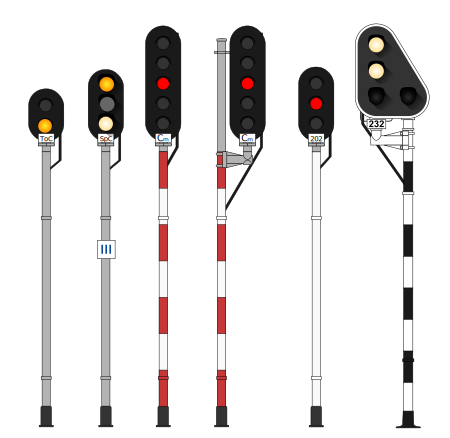
\includegraphics[width=0.45\textwidth]{skryptkierownik-img/sygnalizatory.png}
		\caption{Sygnalizator semafora półsamoczynnego (podg Most Wisła), Sygnalizator samoczynnej blokady liniowej (szlak Pszczyna - Most Wisła), Tarcza ostrzegawcza semafora st. Cz-Dziedzice Południowe, Tarcza przejazdowa ToP na szlaku Bielsko-Biała Leszczyny - Wilkowice-Bystra}
	\end{figure}

\section{Sygnały}
\subsection{Wskazania semaforów półsamoczynnych i samoczynnych}
Sygnalizatory semaforów półsamoczynnych wyposażone są w wiele (3-6)komór sygnałowych oraz dodatkowo mogą być wyposażone w tzw. pas świetlny poniżej komór. Odczyt wskazań semafora zaczynamy zawsze od dołu, dzieląc go umownie na części - górną złożoną z dwóch trzech komór (wskazującą stan następnęgo semafora), oraz dolną z pozostałymi i pasem.

Stanem zasadniczym semaforów półsamoczynnych jest sygnał \textbf{S1 - Stój} - jedno czerwone światło w górnej części semafora. 
Jeśli dolna część semafora jest ciemna, to pominięcie semafora i przejazd przez okręg zwrotnicowy przez niego ochraniany następuje z maksymalną dopuszczalną prędkością (szlakową). 
Jeśli w dolnej części wyświetlane jest światło pomarańczowe wjazd z prędkością do 40 km/h, jeśli poniżej oświetlony jest pas świetlny koloru pomarańczowego - do 60 km/h, zaś jeśli pas jest koloru zielonego - do 100 km/h.
Jeśli w górnej części wyświetlane jest jedno światło pomarańczowe następny semafor wskazuje sygnał Stój, jeśli wyświetlane jest światło zielone - następny semafor zezwala na jazdę z maksymalną dozwoloną prędkością.

\subsection{Tarcze DO i D1}

Tarczę zatrzymania D1 „Stój” ustawia się po prawej stronie toru szlakowego, w odległości 50m przed przeszkodą. W torach stacyjnych tarczę nalezy ustawić w osi toru, 100 m przed przeszkodą. Odległość ta może zostanie skrócona jeśli nie pozwalają warunki miejscowe. W przypadku zamknięcia toru szlakowego pomiędzy posterunkami zapowiadawczymi, nalezy oprocz osygnalizowania przeszkody na miejscu, wystawić tarczę D1 bezpośrednio za ostatnim rozjadem w stacji w kierunku szlaku. Maszyny torowe i pojazdy specjalistyczne osłania się ustawiając tarczę D1 w odległości 3m od maszyny w osi toru.
\ \ Tarczę DO należy ustawić w odległości drogi hamowania zwiększonej o 200m od tarczy D1. W stacjach tarczy DO nie stosuje się.
	\begin{figure}
	\includegraphics[width=0.45\textwidth]{skryptkierownik-img/skryptkierownik-img023.jpg}
	\caption{Tarcza D1 w osi toru}
\end{figure}

\chapter{Przygotowanie drogi przebiegu dla jazd pociągowych i manewrowych}


Droga przebiegu to droga jazdy pomiędzy dwoma kolejnymi sygnalizatorami uzupełniona w miarę potrzeby drogą ochronną oraz urządzeniami ochronnymi. W pierwszej kolejności układa się drogę rozjazdową, poprzez właściwe ustawienie zwrotnic i wykolejnic w terenie, właściwe ustawienie urządzeń zależnościowych takich jak zamki zwrotnicowe i wykolejnicowe, obsługa aparatu blokowego, etc. Następnym krokiem jest zamknięcie (zaryglowanie) a potem utwierdzenie drogi przebiegu, to jest zablokowanie możliwości zmiany ułożenia rozjazdów i wskazań sygnalizatora, do czasu przejechania pociągu poza daną drogę przebiegu.

Przygotowanie drogi przebiegu polega na usunięciu z drogi przebiegu pociągu wszelkiego taboru, przerwaniu manewrów, nastawieniu rozjazdów, oraz zabezpieczeniu przed przypadkowym przełożeniem. Kolejnym etapem jest powiadomienie posterunków dróżników przejazdowych. Ostatnim krokiem jest wyświetlenie sygnałów zezwalających na jazdę manewrową lub pociągową.

\begin{itemize}
	\item Przebieg – przygotowana droga przebiegu z realizacją wszystkich wymaganych uzależnień wraz z podaniem sygnału zezwalającego na jazdę taboru.
	\item Przebieg manewrowy – przebieg dla manewrującego taboru na stacji.
	\item Przebieg pociągowy – przebieg dla pociągu w granicach stacji.
	\item Przebieg niezorganizowany – przebieg, którego droga przebiegu nie jest utwierdzona ani zamknięta.
	\item Przebieg sprzeczny – przebieg, który ze względu bezpieczeństwa nie może być realizowany jednocześnie z innym. 
\end{itemize}

\chapter{Prowadzenie dokumentacji techniczno-ruchowej}

Dyżurny ruchu prowadzi dokumentację techniczno-ruchową w stacji i na przyległych szlakach. 
Podstawowym dokumentem jest dziennik ruchu \textbf{R-146}. Wprowadza się do niego informację o numerze i kierunku (parzysty/nieparzysty), godzinach odjazdu, przyjazdu do posterunku, drodze wolnej. Również uwagi o przejeździe pociągu z TWR, braku sygnałów końca pociągu. Dodatkowo znajdują się tu również informacje o powiadamianiu dróżników przejazdowych. W dzienniku tym umieszcza się również informację o wprowadzeniu ruchu jednotorowego dwukierunkowego.

Książka przebiegów \textbf{R-142} służy do odnotowania poleceń przygotowania wjazdów/wyjazdów dla nastawni wykonawczej. Znajdują się tam informacje o numerze pociągu, torze stacyjnym, oraz godzinach polecenia przygotowania drogi, wyświetlenia semafora.

Dziennik telefoniczny \textbf{R-138} w którym odnotowuje się np. informacje o zgłoszeniu gotowości pociągu, skomunikowaniach, zamknięciu lub otwarciu toru szlakowego. 

Książka urządzeń SRK \textbf{E-1758} w której odnotowuje się wszystkie zdarzenia związane z zerwaniem plomb na urządzeniach, oraz wyświetleniem sygnału zastępczego (które jest rejestrowane licznikiem), a także stanem i usterkami urządzeń SRK. 

Dziennik oględzin rozjazdów \textbf{D-831} w którym odnotowywane są wykonywane przez zwrotniczych lub nastawniczych oględziny i prace w rozjazdach, a także wszelkie uwagi co do ich stanu.

Książka ostrzeżeń doraźnych \textbf{R-189} prowadzona jest dla szlaku(linii kolejowej). Obecnie prowadzona jest w formie elektronicznej przez dyżurnego ruchu.

Kontrolka zajętości torów \textbf{R-292} opisuje stan zajętości torów stacyjnych (wjazdowych) w momencie przyjęcia/zdania dyżuru.

Pozostałe elementy dokumentacji techniczno-ruchowej to rozkazy pisemne ''O'', ''S'',''N'',''Nrob''

\chapter{Rozkazy pisemne i ostrzeżenia dla drużyn pociągowych}

\textbf{Rozkaz pisemny ''O''} - wydaje się w celu przekazania poleceń i informacji dotyczących ostrożnej jazdy, ostrożnej
jazdy z poleceniem zmniejszenia prędkości (np. uszkodzenie SSP, stan SRK, stan drogi kolejowej), Rozkaz pisemny “O”
musi być odebrany przez drużynę pociągową w stacji oznaczonej w wewnętrznym rozkładzie jazdy symbolem “\textbf{R307}”.
Rozkaz pisemny “O” może być wydany na nieustalonym druku (nawet na czystej kartce).  \begin{tcolorbox}[colback=green!5!white,colframe=green!45!black,width=10cm,title=Rozkaz pisemny ''O'']
	W komputerowym wydruku rozkazu pisemnego ''O'' mogą być przekazywane elementy rozkazów ''S'', ''Nrob'' stanowiące \textbf{informacje}
\end{tcolorbox}
 \footnote{Ir-1 Rozdział 8, par. 60, ust. 10)}. 

\textbf{Rozkaz pisemny ''S''} - wydaje się w celu przekazania zezwoleń, poleceń i informacji. Przykładowo wydaje się go w
następujących sytuacjach:

	\begin{figure}
		\includegraphics[width=0.45\textwidth]{skryptkierownik-img/rozkazy-pisemne.jpg}
		\caption{Druki rozkazów pisemnych: od góry ''O'', ''S'', ''N'', ''Nrob''}
	\end{figure}
\begin{itemize}
\item zezwolenie przejechania obok semafora wyjazdowego, wjazdowego, drogowskazowego, wskazującego sygnał “Stój”, sygnał
wątpliwy, białe światło lub nieoświetlonego, jeśli nie można wyświetlić sygnału zastępczego “Sz”.
\item zezwolenie na jazdę manewrową taboru w kierunku szlaku poza ustaloną granicę przetaczania
\item zezwolenie na jazdę w przypadku gdy pojazd trakcyjny znajduje się poza semaforem wskazującym sygnał zezwalający,
którego prowadzący pojazd kolejowy nie widzi.
\item zezwolenie na przejechanie obok tarczy zatrzymania “D1”
\item polecenie jazdy po zamkniętym torze szlakowym i okolicznościach (np. jazda do kilometra i powrót) - w przypadku jazdy na tor zajęty, z przeszkodą, z prędkością do 30 km/h, na tor wolny z prędkością rozkładową.
\item polecenie nie przewidzianego w rozkładzie jazdy zatrzymania pociągu, z określeniem celu i czasu postoju
\item informacja o ustawieniu nowych lub zmianie ustawienia sygnalizatora (przez 14 dni)
\item informacja o jeździe pociągu w innym kierunku niż przewidziany w w.r.j.
\end{itemize}

\textbf{Rozkaz pisemny ''N'' } - wydaje się drużynie pociągowej w celu przekazania zezwoleń, poleceń i informacji o wyjeździe pociągu na tor szlakowy lewy ( w kierunku przeciwnym do zasadniczego), gdy semafor wyjazdowy wskazuje sygnał ''Stój'', o wjeździe pociągu z toru lewego i co będzie sygnałem zezwalającym na wjazd, informację o tym że przejazd pociągu po torze lewym obok posterunków odstępowych może nastąpić po otrzymaniu ręcznego sygnału Rm1 “Do mnie” od dyżurnego, zawsze wtedy gdy ruch prowadzony jest jednotorowo, dwukierunkowo, a tor zasadniczy dla tego kierunku ruchu  jest zamknięty.

W czasie planowych zamknięć torów, w celu wykonania robót, drużynie pociągowej potrzebne zezwolenia, polecenia i informacje mogą być wydawane za pomocą \textbf{rozkazu pisemnego ''Nrob''}. Informacje i zezwolenia dyżurny ruchu wprowadza na podstawie regulaminu tymczasowego, wydawanego na czas robót.

Rozkazy pisemne wystawia dyżurny ruchu dysponujący danego posterunku, zaś techniczną czynność wypisania i doręczenia rozkazu może wykonać inny, upoważniony pracownik (np. zwrotniczy, nastawniczy, etc.), na \textbf{polecenie} dyżurnego ruchu. Jeśli posterunek ruchu jest wyposażony w urządzenia rejestrujące połączenia telefoniczne i radiowe (w rozkładzie przy stacji symbol \textbf{RT}), rozkaz pisemny może być przekazany drogą radiotelefoniczną, w czasie biegu pociągu (wyłącznie przy dwuosobowej obsadzie drużyny trakcyjnej i poniżej 130 km/h).

Numeracja rozkazów pisemnych w bloczku prowadzona jest w porządku rocznym. Jeśli rozkaz przekazywany jest drogą radiotelefoniczną, to na druku znajdującym się na pojeździe trakcyjnym należy numer rozkazu wpisywać wg podwójnej numeracji - (jako pierwszy numer kolejny na pojeździe, a następnie numer na posterunku ruchu)

\chapter{Wewnętrzny rozkład jazdy}

\section{Elementy rozkładu jazdy}
Rozkład jazdy pociągów to podstawowy element organizacji przewozów kolejowych stanowiący plan pracy kolei, według którego odbywa się ruch wszystkich pociągów po sieci kolejowej lub jej części.  Rozkład jazdy prezentowany jest jako karty rozkładu jazdy. Każda karta rozkładu jazdy, składa się ze strony tytułowej oraz szczegółowego rozkładu jazdy dla pociągu. Aktualnie istnieją dwa dodatki do wewnętrznego rozkładu jazdy:
\begin{tcolorbox}[colback=green!5!white,colframe=green!75!black,width=0.47\textwidth,title=Dodatki do rozkładu jazdy]
\begin{itemize}
	\item Dodatek 1. do WRJ zawiera Warunki techniczno-ruchowe linii kolejowych zarządzanych przez PLK. Dodatek 1. do WRJ jest
	opracowywany okresowo.
	\item Dodatek 2. do WRJ zawiera wykaz ostrzeżeń stałych oraz prędkości drogowych na torach głównych zasadniczych stacji
	węzłowych. Dodatek 2. do WRJ jest opracowywany okresowo, przy czym po raz pierwszy równocześnie z wejściem w życie rocznego RJ.
\end{itemize}
\end{tcolorbox}
Ostrzeżenia dzielą się na \textbf{stałe} i \textbf{doraźne}. Ostrzeżeniami doraźnymi są ostrzeżenia nie ujęte w wykazie ostrzeżeń stałych. W wykazie ostrzeżeń stałych należy wskazać wszystkie ostrzeżenia, które trwać będą dłużej niż 30 dni.
W wykazie ostrzeżeń stałych umieszczone są odstępstwa od rozkładu jazdy, takie jak ograniczenia prędkości, zachowanie szczególnej ostrożności. Zmiany w WOS wprowadzane są w postaci "poprawek". Mogą one dotyczyć wyłącznie zmniejszenia dolegliwości ograniczenia, np. skreślenia całości ograniczenia, skrócenia kilometrażu objętego ograniczeniem, czy zwiększenia prędkości. Poprawką do WOS nie może być wprowadzone zmniejszenie prędkości. 
Wewnętrzny rozkład jazdy tworzony jest w formie tabeli. \begin{figure}
	\includegraphics[width=0.45\textwidth]{skryptkierownik-img/numer-linii.png}
	\caption{Numer linii oraz kilometraż}
\end{figure} W kolumnie pierwszej znajduje się numer linii zgodnie z wykazem linii PKP PLK. W kolumnie drugiej znajduje się kilometraż początku i końca danego odcinka linii (strona lewa), oraz kilometraż zmiany prędkości rozkładowej (strona prawa). 

\begin{table}
	\begin{tabular}{|c|m{4cm}|c|m{4cm}|}
		\hline 
		m & stacja mijanka & Rd1 & zezwolenie na wyjazd pociągu pasażerskiego - obowiązuje sygnał Rd1 "Nakaz Jazdy" \\ 
		\hline
		skp & posterunek stwierdzania końca pociągu & R1& Numer kanału radiołączności\\ 
		\hline
		po	& przystanek osobowy & H & zainstalowane są urządzenia SHP\\ 
		\hline
		podg	& posterunek odgałeźny &  R307	& posterunek z którego nie można odjechać, bez otrzymania rozkazu pisemnego 'O'\\ 
		\hline
		pt	& postój techniczny & zp & zatrzymanie dla zabrania pracowników (post. ruchu)\\ 
		\hline
		\textbf{Stacja}	& Nazwa stacji & \textbf{STACJA} & Nazwa stacji węzłowej \\ 
		\hline
		W24	& \multicolumn{3}{m{9cm}|}{posterunek na którym zezwoleniem na wyjazd na tor szlakowy lewy jest sygnał zezwalający lub Sz wraz z wyświetlonym wskaźnikiem W24} \\
		\hline
	\end{tabular} 
	\caption{Objaśnienia znaków i skrótów (str. stałe) w.r.j - opisy stacji}
\end{table}
W kolumnie trzeciej znajduje się informacja o prędkości rozkładowej (drogowej) odcinka linii, a także po którym torze został opracowany rozkład.
\begin{figure}
	\includegraphics[width=0.45\textwidth]{skryptkierownik-img/tor-lewy.png}
	\caption{Wskazanie po którym torze opracowano rozkład i prędkości rozkładowe}
\end{figure}

W kolumnie czwartej znajdują się nazwy posterunków ruchu przez które pociąg ma przejeżdżać, wraz z opisem technicznym (typ postoju, numer kanału radiowego). Opis w polu stacji zawiera również informacje o rodzaju blokady na który nastąpi wyjazd na tor szlakowy. 
\begin{table}
	\begin{tabular}{|c|m{11cm}|}   
		\hline
		PP	& blokada półsamoczynna przystosowana do jazdy po torze lewym (przeciwnym do zasadniczego) \\ 
		\hline
		S	& blokada samoczynna na szlaku jednotorowym, lub samoczynna jednokierunkowa w kierunku zasadniczym \\ 
		\hline
		SS	& blokada samoczynna przystosowana do jazdy po torze lewym (przeciwnym do zasadniczego) \\ 
		\hline
		SP	& dla kierunku zasadniczego blokada samoczynna, dla toru kierunku przeciwnego półsamoczynna \\ 
		\hline
		PS	& blokada półsamoczynna dla jazdy pociągu w kierunku zasadniczym, blokada samoczynna przystosowana do jazdy po torze lewym (przeciwnym do zasadniczego) \\ 
		\hline
	\end{tabular} 
	\caption{Przystosowanie blokady liniowej do ruchu dwukierunkowego}
\end{table}
W kolumnie piątej znajduje się informacja o godzinie przyjazdu i odjazdu dla danego posterunku. Jeśli w polu znajduje się tylko jedna godzina, oznacza to że nie jest przewidywany postój na tym posterunku. W tej samej kolumnie znajduje się również informacja o zmianie numeru pociągu (np. zmiana kierunku jazdy). W pozostałych kolumnach wskazane są informacje o taborze planowym, masie brutto, długości pociągu, prędkości maksymalnej taboru, oraz procencie wymaganym masy hamującej.
\begin{figure}
	\includegraphics[width=0.45\textwidth]{skryptkierownik-img/rozklad-odjaz.png}
	\caption{Rozkładowa godzina odjazdu pociągu}
\end{figure}


\section{Numeracja pociągów}

Pociągi pasa­żerskie krajowe ozna­czane są nume­rami cztero- i pięcio­cyfro­wymi, a pociągi towa­rowe krajowe, utrzymaniowo-naprawcze i niehan­dlowe nume­rami sześcio­cyfro­wymi. Numer pociągu ma być jedno­lity i ma nie zmieniać się na całej trasie pociągu. Numery pociągów międzynaro­dowych usta­lane mają być według odrębnych zasad.

Pierwsza i druga cyfra w numerach cztero-, pięcio- i sześciocyf­rowych określa obszar konstruk­cyjny urucho­mienia i rozwią­zania pociągu. Obszary konstruk­cyjne ozna­czone są nastę­pują­cymi numerami:

1 - Warszawa,\\
2 - Lublin,\\
3 - Kraków,\\
4 - Sosnowiec,\\
5 - Gdańsk,\\
6 - Wrocław,\\
7 - Poznań,\\
8 - Szczecin,\\
9 - rezerwa.\\

Dla pociągów rozpoczyna­jących i kończących bieg wewnątrz jednego obszaru konstrukcyj­nego stoso­wane mogą być następu­jące kombi­nacje dwóch pierwszych cyfr numeru:

11, 10, 19, 91 - Warszawa,\\
22, 20, 29 - Lublin,\\
33, 30, 39, 93 - Kraków,\\
40, 44, 90, 94, 99 - Sosnowiec,\\
55, 50, 59, 95, 96, 97 - Gdańsk,\\
66, 60, 69 - Wrocław,\\
77, 70, 79 - Poznań,\\
88, 80, 89 - Szczecin,\\
92, 98 - rezerwa.\\
Pozostałe cyfry ozna­czają rodzaj pociągu i nada­wane być powinny zgodnie z kolej­nością urucha­miania pociągów w dobie.
\begin{figure}
	\includegraphics[width=0.5\textwidth]{skryptkierownik-img/obszary-konstrukcyjne.png}	
	\caption{Obszary konstrukcyjne rozkładu jazdy}
\end{figure}

\chapter{Nadzór nad prowadzeniem i regulowaniem ruchu pociągów w sytuacjach nadzwyczajnych}

Rozkłady jazdy ustalane są tak, by zachowana została kolejność pierwszeństwa przejazdu według rodzaju i kategorii pociągów. 
Naczelną zasadą jest, że pierwszeństwo mają pociągi pasażerskie nad towarowymi. Rozpatrując pociągi pasażerskie to kryterium pierwszeństwa jest prędkość jazdy w związku z czym wyodrębnia się w kolejności od najwyższego stopnia pierwszeństwa pociągi: 
\begin{enumerate}
	\item nadzwyczajne specjalnego znaczenia, 
	\item kwalifikowane (EC, IC, Ex),
	\item pociągi pośpieszne,
	\item pociągi osobowe i aglomeracyjne dowożące ludzi do pracy, 
	\item pociągi osobowe i dalekobieżne i pozostałe miejscowe itd. 
\end{enumerate}
W sytuacjach nadzwyczajnych pierwszeństwo ponad wszystkimi z tych pociągów mają pociągi ratunkowe. Drezyny na blokadzie samoczynnej zawsze jako telefoniczne zapowiadanie pociągów. 

\chapter{Organizacja akcji ratunkowej w razie zdarzeń kolejowych i klęsk żywiołowych}

\section{Podstawowe pojęcia}

\textbf{Wydarzenie kolejowe} – każda niepożądana sytuacja zaistniała w systemie transportu kolejowego lub w jego otoczeniu zakłócająca realizację procesu przewozowego, w szczególności powodująca zagrożenie dla bezpieczeństwa ruchu kolejowego, opóźnienie pociągu lub zakłócenie prac manewrowych.
\\
\textbf{Wypadek} \footnote{Instrukcja Ir-8, \S.2, pkt.6}– niezamierzone nagłe zdarzenie lub ciąg takich zdarzeń z udziałem pojazdu kolejowego, powodujące negatywne konsekwencje dla zdrowia ludzkiego, mienia lub środowiska; 
do wypadków zalicza się w szczególności:
\begin{enumerate}
	\item kolizje;
	\item wykolejenia;
	\item zdarzenia na przejazdach;
	\item zdarzenia z udziałem osób spowodowane przez pojazd kolejowy będący w ruchu;
	\item pożar pojazdu kolejowego.
\end{enumerate}
\textbf{Poważny wypadek} – każdy wypadek spowodowany kolizją, wykolejeniem lub innym
zdarzeniem mającym oczywisty wpływ na regulacje bezpieczeństwa kolei lub na
zarządzanie bezpieczeństwem:
\begin{itemize}
	\item z przynajmniej \textbf{jedną} ofiarą \textbf{śmiertelną} lub przynajmniej \textbf{pięcioma ciężko rannymi};
	lub
	\item powodujący znaczne \textbf{zniszczenie pojazdu} kolejowego, infrastruktury kolejowej lub środowiska, które mogą zostać \textbf{natychmiast oszacowane} przez komisję badającą wypadek na co najmniej \textbf{2 miliony euro}.
\end{itemize}
\textbf{Znaczący wypadek} – wypadek z udziałem co najmniej jednego pojazdu kolejowego
będącego w ruchu:
\begin{itemize}
\item \textbf{z przynamniej jedną} ofiarą śmiertelną lub ciężko ranną;
lub
\item powodujący \textbf{znaczne szkody} w taborze, torach kolejowych, instalacjach lub
środowisku, tj. szkodę o wartości \textbf{co najmniej 150 tysięcy euro};
lub
\item powodujący znaczne zakłócenie ruchu, tj. wstrzymanie ruchu kolejowego na głównej linii kolejowej przez co najmniej 6 godzin.
\end{itemize}

\textbf{Incydent} – każde zdarzenie inne niż wypadek lub poważny wypadek, związane z ruchem kolejowym i mające wpływ na jego bezpieczeństwo.

\textbf{Sytuacja potencjalnie niebezpieczna} – sytuacja eksploatacyjna lub wydarzenie kolejowe niebędące poważnym wypadkiem, wypadkiem ani incydentem, powodujące nieznaczny wzrost ryzyka – do kontrolowanego poziomu nieprzekraczającego poziomu ryzyka akceptowalnego.

\section{Postępowanie przy zdarzeniu}
Postępowanie przy organizacji i prowadzeniu akcji ratunkowej określają instrukcje PKP PLK (Ir-8),instrukcje wewnętrzne KŚ (K-6, K-9), oraz procedura SMS P-16.
\\Pracownik kolejowy, który zauważył, że może dojść do zdarzenia, powinien użyć wszelkich możliwych środków, aby mu zapobiec, a gdy to jest niemożliwe, dążyć do ograniczenia jego skutków. 
W przypadku zabicia lub zranienia człowieka przez pojazd kolejowy, pojazd ten należy zatrzymać, a kierownik pociągu lub maszynista (albo ewentualnie inny pracownik kolejowy) zgłasza zdarzenie dyżurnemu ruchu na najbliższym posterunku ruchu zarządcy infrastruktury.
\footnote{Instrukcja Ir-8, Rozdział II, \S.5}
\\Do czasu przybycia na miejsce zdarzenia naczelnika sekcji eksploatacji lub wyznaczonego przez niego pracownika, pracownik kolejowy, który zauważył zdarzenie, a w szczególności \textbf{kierownik pociągu}, czy prowadzący pojazd kolejowy, powinien:
\begin{enumerate}
	\item \textbf{poinformować dyżurnego ruchu} na najbliższym posterunku ruchu zarządcy infrastruktury o nieplanowym zatrzymaniu na szlaku, podając numer pociągu, szlak i kilometr, oraz prawdopodobną przyczynę, oraz o dostrzeżonych zagrożeniach dla dalszego prowadzenia ruchu kolejowego, spowodowanych zaistniałym zdarzeniem;
	\item sprawdzić, czy na sąsiednich torach może odbywać się ruch pociągów (manewry).
	Jeżeli ruch nie może się odbywać, należy, o ile to możliwe, zabezpieczyć miejsce zdarzenia, a do zbliżających się pociągów podawać sygnał „Alarm”;
	\item udzielić pierwszej pomocy poszkodowanym;
	\item przeciwdziałać powstaniu i rozprzestrzenianiu się pożaru;
	\item zabezpieczyć ślady mogące mieć znaczenie dla ustalenia przyczyn zdarzenia i nie dopuścić do ich zatarcia;
	\item zabezpieczyć mienie kolejowe, ładunki i bagaże pasażerów;
	\item informować dyżurnego ruchu o fakcie i czasie przybycia na miejsce zdarzenia służb	ratowniczych oraz ich rodzaju (pogotowie ratunkowe, straż pożarna, policja, zespół kolejowego ratownictwa technicznego itp.).
\end{enumerate}

\section{Pożar}
\footnote{Instrukcja K-9, Rozdział II, \S.4, ust 1-9}
W razie powstania pożaru w pociągu należy pociąg ten niezwłocznie zatrzymać, podawać sygnał „Pożar”, wezwać podróżnych do opuszczenia palącego się wagonu i starać się ugasić pożar za pomocą posiadanych środków, w razie potrzeby przy pomocy podróżnych. Jeżeli nie można ugasić pożaru w zarodku, należy wezwać straż pożarną. Obowiązkowo o pożarze powiadomić dyżurnego ruchu, a w razie potrzeby miejsce niebezpieczne osłonić sygnałami i zażądać pomocy.

\section{Wykolejenie}
Wykolejenie jest to  trwała utrata kontaktu powierzchni tocznej koła pojazdu kolejowego z powierzchnią toczną główki szyny.
W razie wykolejenia, kierownik pociągu \textbf{natychmiast zawiadamia} dyżurnego ruchu najbliższego posterunku ruchu.
Gdy zajdzie taka potrzeba żąda przybycia karetki pogotowia, a rannym podróżnym, z udziałem pozostałych członków drużyny konduktorskiej - udziela pierwszej pomocy. Kierownik pociągu za każdym razem określa, czy wykolejone wagony nie stanowią zagrożenia dla bezpieczeństwa ruchu prowadzonego po torach sąsiednich. W razie zdarzenia kolejowego z udziałem pociągu z materiałami niebezpiecznymi, materiałami szczególnie niebezpiecznymi i wybuchowymi, kierownik pociągu bezwzględnie zawiadamia dyżurnego ruchu najbliższego posterunku ruchu informując go o tym fakcie i żądając wstrzymania ruchu na szlaku na którym nastąpił wypadek.
\footnote{Instrukcja Ir-1, Rozdział 10, \S.76, ust 2}

Wagony wykolejone, nawet nie uszkodzone, powinny być zbadane przez \textbf{rewidenta} taboru kolejowego przed dopuszczeniem ich do dalszej jazdy w pociągu. W razie niemożności dokładnego zbadania wagonów wykolejonych na szlaku, po wstawieniu ich na tor, należy dowieźć je do najbliższej stacji, dostosowując prędkość jazdy do wskazówek rewidenta taboru kolejowego, przy czym prędkość ta nie może być większa niż 30 km/h.

\chapter{Obowiązki manewrowego oraz nadzorującego i kierującego manewrami}

Kierownikiem manewrów może być: \textbf{ustawiacz, kierownik pociągu, dyżurny ruchu, nastawniczy, zwrotniczy}. 

Zespół pracowników zlożony z kierownika manewrów i co najmniej jednego pracownika manewrowego,  nazywa się drużyną
manewrową. Prowadzący pojazd kolejowy oraz pracownik posterunku nastawczego powinni zostać powiadomieni kto jest
kierownikiem manewrów. Pracownicy biorący udział w manewrach powinni znać regulaminy techniczne oraz pracy obsługiwanej
bocznicy kolejowej, dla rejonu w którym wykonują manewry.

Do obowiązków kierownika manewrów należy:

\begin{itemize}
\item ustalenie pracy manewrowej, omówienie z drużyną trakcyjną oraz obsługą posterunków nastawczych
\item podział czynności między manewrowych
\item sprawdzenie stanu zajętości i zamknięcia torów
\item sprawdzenie zabezpieczenia pojazdów kolejowych przed zbiegnięciem
\item sprawdzenie stanu i liczby płozów hamulcowych, oświetlenia i łączności
\item kierowanie rozrządzaniem i zestawieniem pociągów
\item dawanie sygnałów manewrowych
\item sprzęganie i rozprzęganie pojazdów
\end{itemize}
\ \ Kierownik manewrów może jednoosobowo wykonywać następujące manewry:

\begin{enumerate}
\item z włączonym hamulcem zespolonym
\end{enumerate}
\begin{itemize}
\item \begin{itemize}
\item przestawiać próżne składy pasażerskiego
\item przestawiać próżne zespoły trakcyjne – maszynista powinien prowadzić pojazd z pierwszej kabiny patrząc w kierunku
jazdy
\item wyciągać bez zmiany kierunku jazdy składy towarowe z torów przyjazdowych na wyciągowe, z torów kierunkowych na
odjazdowe.
\item Przestawiać z toru na tor składy nie przekraczające 60 osi rzeczywistych, na sygnały manewrowe na sygnalizatorach,
gdy pojazd trakcyjny i pracownik manewrowy posiadają sprawny radiotelefon, bez ograniczeń długości.
\end{itemize}
\end{itemize}
\begin{enumerate}
\item bez hamulca zespolonego przestawiać grupy wagonów do 8 osi rzeczywistych (ładowne), 28  osi rzeczywistych (próżne)
\item Nie wolno odrzucać pojazdów kolejowych w pojedyńczej obsadzie manewrowej
\end{enumerate}
\ \ Składy pociągów należy zostawić w stanie ściśniętych sprężyn zderzakowych, z zakręconym hamulcem ręcznym na
pierwszym i ostatnim wagonie.

\ \ Po zakończeniu manewrów, do obowiązków kierownika pociągu należy sprawdzenie czy pojazdy kolejowe znajdują się w
granicach ukresów oraz czy są należycie zabezpieczone przed zbiegnięciem.

\ \ Obowiązki manewrowego przed rozpoczęciem pracy:

\begin{itemize}
\item zgłoszenie się u kierownika manewtów, z przepisowym wyposażeniem (ochrona osobista i sygnałowe)
\item sprawdzenie stanu zapełnienia trów i które tory są wolne
\item czy pojazdy kolejowe są dopchnięte i połączone sprzęgami
\item czy pod kołami pojazdów nie ma płozów, lub innych przeszkód (np. wykolejnica)
\item czy na torach nie znajdują się pojazdy uszkodzone, wykolejone, z ładunkiem przesuniętym, uszkodzonym, lub pojazdy
wymagające zachownia szczególnej ostrożnością
\item sprawdzenie czy nie ma przeszkód na przejazdach kolejowo-drogowych (pojazdy, lód, piasek, zanieczyszczenia w
żłobkach)
\end{itemize}

\ \ W trakcie wykonywania manewrów obowiązki manewrowego to m.in.:

\begin{itemize}
\item rozprzęganie i sprzęganie pojazdów
\item przestawianie zwrotnic i wykolejnic przewidzianych do obsługi przez drużynę manewrową
\item dawanie sygnałów manewrowych
\item hamowanie manewrujących pojazdów
\item zabezpieczenie przed zbiegnięciem
\end{itemize}

\ \ Manewrowy może podawać sygnały przed dojechaniem do wagonów które ma połączyć, na polecenie kierownika manewrów,
albo celem wstrzymania manewrów w razie niebezpieczeństwa.

\ \ Po zakończeniu manewrów powinien sprawdzić czy nie pozostawiono pojazdów poza ukresem, zabezpieczyć pojazdy przed
zbiegnięciem, nieużyte płozy złożyć w wyznaczynm miejscu, pozawieszać sprzęgi hamulcowe na wsporniki.

\chapter{Sposoby wykonywania manewrów}

\textbf{\ \ Manewry} są to wszelkie zamierzone ruchy pojazdów kolejowych oraz związane z nimi czynności na torach, z wyjątkiem wjazdu, wyjazdu i przejazdu pociągów.
\footnote{Instrukcja Ir-1, Rozdział II, \S.11, pkt.1}

\ \ Manewry prowadzi się na trzy sposoby:

\begin{itemize}
\item \textbf{Odstawianie} polegające na przestawianiu pojazdów kolejowych na wyznaczony tor i odczepieniu po
zatrzymaniu, pojazdem trakcyjnym, podciągarką, przesuwnicą wagonową.
\item \textbf{Odrzucanie} polegające na tym że lokomotywa manewrowa pchając odprzęgnięte wagony, przy pewnej, określonej
prędkości zatrzymuje się, co powoduje że odprzęgnięte od niej wagony toczą się dalej samodzielnie na wyznaczony tor
\item \textbf{Grawitacyjny} polegający na staczaniu wagonów z gorki rozrządowej lub torów położonych na spadku
\end{itemize}

Wszelkie manewry należy wykonywać po uzgodnieniu z dyżurnym ruchu, oraz przerwać na każde jego żądanie. 

Bez drużyny manewrowej może odbywać się jazda manewrowa pojazdów pomocniczych, jazda manewrowa taboru specjalnego, jazda manewrowa pojazdów trakcyjnych bez doczepionego taboru, jazda manewrowa pojazdów trakcyjnych \textbf{ciągnących} nie więcej niż cztery wagony towarowe albo \textbf{dwa wagony} pasażerskie bez \textbf{podróżnych}, jazda manewrowa próżnych składów złożonych z zespołów trakcyjnych, przejazd ciągnionych składów pociągowych z torów przyjazdowych do innego rejonu stacji oraz z torów kierunkowych na tory odjazdowe, jazda manewrowa lokomotywy \textbf{pchającej} dwa wagony towarowe albo jeden \textbf{wagon pasażerski bez podróżnych}, gdy drużyna trakcyjna jest dwuosobowa, podstawienie pod perony \textbf{próżnych składów} pasażerskich prowadzonych z przedniej kabiny patrząc w kierunku jazdy.

Nie wolno odrzucać następujących wagonów:

\begin{itemize}
\item wagony z podróżnymi,
\item wagony salonowe, doświadczalne, laboratoryjne, pomiarowe, wagowe, podstacje elektryczne, inne służące różnym celom np.:
gospodarczym, socjalnym itp.
\item 
nieczynne pojazdy trakcyjne,
\item 
pojedyncze wagony ciężkie o masie brutto większej niż 120 ton,
\item wagony załadowane przesyłką przekraczającą skrajnię ładunkową lub przesyłką o masie ponad 60 ton w jednej sztuce oraz
wagony załadowane kontenerami wielkimi (o długości 6 m i większej),
\item wagony ogrzewcze, wagony z czynnym ogrzewaniem piecowym oraz wagony uszkodzone oznaczone nalepkami oznaczającymi
nieprzydatność wagonu do biegu na własnych kołach,
\item pojazdy specjalne np. żurawie kolejowe, maszyny do robót torowych, pługi odśnieżne itp.,
\item wagony bez ław pokrętnych z ładunkiem leżącym na dwu lub więcej wagonach (np.: długie szyny, pręty stalowe i inne długie
elastyczne przedmioty), 
\item wagony oznaczone nalepką ostrzegawczą nr 8 lub 15 według RID,
\begin{figure}
	\includegraphics[width=0.35\textwidth]{skryptkierownik-img/znaki-manewrowania.png}
	\caption{Nalepki ostrzegawcze nr 13 ostrożnie przetaczać oraz nr 15 zakaz odrzutu i staczania} 
	\end{figure}
\item wagony cysterny oznaczone pasem koloru pomarańczowego, 
\item wagony do przewozu podróżnych, sypialne i restauracyjne oraz pocztowe i bagażowe.
\end{itemize}
Stałe oznaczenia i napisy ostrzegawcze na wagonach wymagających zachowania szczególnej ostrożności przy wykonywaniu nmanewrów

(kolor biały, umieszczone na ostojnicy z lewej strony):

\textbf{1. Znak ostrzegawczy}- zabroniony przejazd przez górkę rozrządową;
\begin{figure}
	\includegraphics[width=0.25\textwidth]{skryptkierownik-img/skryptkierownik-img024.jpg}
	\caption{Znak ostrzegawczy - zakaz przejazdu przez górkę rozrządową}
\end{figure}

\textbf{2. Znak ostrzegawczy} - zabroniony przejazd przez górkę rozrządową o promieniu krzywizny (w płaszczyźnie pionowej) mniejszym, niż podany pod znakiem;
\begin{figure}
	\includegraphics[width=0.25\textwidth]{skryptkierownik-img/skryptkierownik-img025.jpg}
	\caption{Znak ostrzegawczy - zabroniony przejazd przez górkę o promieniu krzywizny}
\end{figure}
\textbf{3. Znak ostrzegawczy}- dopuszcza się przetaczanie przez górkę rozrządową tylko przy zachowaniu szczególnych środków ostrożności:
\begin{figure}
	\includegraphics[width=0.25\textwidth]{skryptkierownik-img/skryptkierownik-img026.jpg}
	\caption{Znak ostrzegawczy - zachowanie ostrożności}
\end{figure}

Na tor \textbf{prawy} - zasadniczy szlaku dwutorowego przy ruchu dwutorowym jednokierunkowym zezwolenie \textbf{ustne} wykonania manewrów może udzielić dyżurny ruchu. Na tor \textbf{przeciwny} do zasadniczego zezwolenie wykonania manewrów musi być udzielone na podstawie \textbf{rozkazu pisemnego ''S''}. Zezwolenie takie może być wydane na wielokrotne jazdy w ściśle określonym obrębie czasu. Każdorazowo poza zezwoleniem musi być podany sygnał manewrowy podawany na sygnalizatorze lub sygnał ręczny "Do mnie".

\chapter{Sygnały podawane przy manewrach}

\section{Tarcze manewrowe świetlne i kształtowe}
Podstawowe sygnały manewrowe Ms1 i Ms2 podawane są przy pomocy tarcz manewrowych świetlnych. Na niektórych posterunkach mogą istnieć również tarcze manewrowe kształtowe lub nieruchome. Jeśli występuje tarcza manewrowa nieruchoma, podająca sygnał ''M1 Jazda manewrowa zabroniona'', należy pojazd kolejowy zatrzymać przed tarczą, a dalszą jazdę manewrową można kontynuować na polecenie ustne dyżurnego ruchu i sygnał Rm1 ''Do mnie''.
\begin{figure}
	\includegraphics[width=0.25\textwidth]{skryptkierownik-img/tarcza-manewrowa-ms1.jpg}
	\caption{Tarcza manewrowa karzełkowa wskazująca sygnał Ms1}
\end{figure}
 W przypadku tarcz kształtowych ruchomych, oraz sygnalizatorów świetlnych, zezwoleniem na wykonywanie manewrów taboru jest sygnał ''Ms2 Jazda manewrowa dozwolona'' (jedno matowobiałe światło na tarczy/semaforze). Jeśli nie można na sygnalizatorze nastawić sygnału M2 lub Ms2, manewrujący może przejechać poza sygnalizator zabraniający dalszej jazdy, gdy upoważniony pracownik da zezwolenie na jazdę (ustnie, radiotelefonicznie) oraz sygnał odpowiednio Rm1 ''Do mnie'' lub Rm2 ''Ode mnie''.

\section{Semafory półsamoczynne lub tarcze zaporowe}
Na semaforach półsamoczynnych przystosowanych do podawania sygnałów manewrowych (oznaczonych literą m na tabliczce z nazwą semafora) istnieje możliwość podania sygnału Ms2. Sygnału Ms1 nie wyświetla się na takim semaforze, w jego miejsce podawany jest sygnał S1 ''Stój''

\section{Sygnały ręczne i dźwiękowe}
\begin{itemize}
\item \textbf{Rm1 Do mnie}
Sygnał ''Do mnie'' podaje się chorągiewką sygnałową koloru żółtego lub ręką poruszaną poziomo, oraz przy pomocy gwizdawki - dwa długie tony.
\item \textbf{Rm2 Odemnie}
Sygnał ''Ode mnie'' podaje się chorągiewką sygnałową koloru żółtego lub ręką poruszaną pionowo, oraz przy pomocy gwizdawki - jeden długi ton.
\item \textbf{Rm3 Zwolnić}
Sygnał ''Zwolnij'' podaje się chorągiewką sygnałową koloru żółtego lub ręką poruszaną po łuku do góry i na dół, oraz przy pomocy gwizdawki - kilka przeciągłych tonów.
\item \textbf{Rm6 Docisnąć}
Sygnał ''Docisnąć'' podaje się poprzez kilkukrotne zbliżenie do siebie wyciągniętych poziomo przed siebie rąk, oraz przy pomocy gwizdawki - dwa krótkie tony.
\item \textbf{Rm4 Stój}
Sygnał ''Stój'' podajemy wykonując okrężny ruch wyprostowaną reką, chorągiewką sygnałową, lub w nocy latarką, oraz przy pomocy gwizdawki podając wielokrotnie trzy krótkie dźwięki. Sygnał ''Stój'' podaje się aż do całkowitego zatrzymania pojazdu.
\end{itemize}


\chapter{Prędkości jazd manewrowych i pociągowych}
\begin{table}
\begin{tabular}{|c|c|}
\hline
Opis &
Prędkość dopuszczalna\\\hline
Jazda pociągu na tor zamknięty - bez przeszkody, po otrzymaniu tej informacji na rozkazie pisemnym S &
z prędkością rozkładową\\\hline
Jazda manewrowa po torze wolnym (bez rozjazdów), po omówieniu pracy manewrowej &
40 km/h\\\hline
Wyjazd na sygnał zastępczy na szlak z półsamoczynną blokadą liniową (do granicy posterunku) &
40 km/h\\\hline
Odjazd pociągu z krawędzi przyperonowej, gdy nie widać wskazań semafora &
40 km/h\\\hline
Cofanie pociągu ze szlaku po uzgodnieniu z dyżurnym ruchu &
30 km/h\\\hline
Jazda pociągu na tor zamknięty - zajęty (z przeszkodą) &
30 km/h\\\hline
\textbf{Zasadnicza prędkość~manewrowa} &
25 km/h\\\hline
Przez niezabezpieczone przejazdy i przejścia &
20 km/h\\\hline
Na torze zamkniętym, na 500m przed przeszkodą &
20 km/h\\\hline
Wyjazd na sygnał zastępczy na szlak z samoczynną blokadą liniową (do następnego semafora) &
20 km/h\\\hline
Wjazd do stacji na tor zakończony kozłem oporowym, lub niedostępny w części &
20 km/h\\\hline
Manewry na tor częściowo zajęty &
20 km/h\\\hline
Jazdy składu manewrowego pojazdami kolejowymi naprzód po torze głównym o spadku ponad 2,5\textperthousand, a pojazd trakcyjny nie mógł być umieszczony od strony spadku &
15 km/h\\\hline
Z podróżnymi, z towarami niebezpiecznymi, z przesyłką nadzwyczajną &
10 km/h\\\hline
Dojeżdżanie odsprzęgów staczanych z górki do stojącego taboru &
5,4 km/h\\\hline
Nieuzgodnione cofanie pociągu ze szlaku poprzedzone w drodze hamowania przez pracownika drużyny &
5 km/h\\\hline
Na sygnał „ pchać z umiarkowaną szybkością”, przy rozprzęganiu drążkiem, przy przetaczaniu wagonów oznaczonych nalepką ostrzegawczą 8 lub 15 wg RID oraz cystern z pasem koloru pomarańczowego, jeśli pracownik manewrowy porusza się przedskładem &
5 km/h\\\hline
Na sygnał „pchać powoli”, przy dojeżdżaniu lokomotywy do stojącego taboru, przy przetaczaniu za pomocą urządzeń
mechanicznych &
3 km/h\\\hline
Przy dojeżdżaniu do stojących pojazdów kolejowych &
3 km/h\\\hline
\end{tabular}
\end{table}
\chapter{Manewry po torach głównych oraz przez przejazdy i przejścia}

Manewry po torach głównych można wykonywać wyłącznie za zgodą dyżurnego ruchu nastawni dysponującej. Wyjazd manewrującego taboru na szlak (w kierunku szlaku) poza
wskaźnik oznaczający granicę przetaczania, a gdzie wskaźnika takiego nie ma – poza ostatni rozjazd (skrzyżowanie torów),dozwolony jest tylko za zezwoleniem dyżurnego ruchu.

W przypadku wyjazdu na tor (w kierunku toru):

– szlaku jednotorowego,

– lewy szlaku dwutorowego (w kierunku przeciwnym do zasadniczego),

– prawy szlaku dwutorowego (w kierunku zasadniczym), po którym prowadzony jest ruch dwukierunkowy,

– w kierunku przeciwnym do zasadniczego szlaku wielotorowego,

– w kierunku zasadniczym, po którym prowadzony jest ruch dwukierunkowy szlaku wielotorowego, zezwolenie to musi być przekazane rozkazem pisemnym „S”

\ \ Na tor prawy (\textbf{zasadniczy}) szlaku \textbf{dwutorowego}, gdy prowadzony jest po nim ruch \textbf{jednokierunkowy} jazda za wskaźnik granicy przetaczania możliwa jest na ustne zezwolenie dyżurnego ruchu.

Manewry przez przejazdy i przejścia kolejowo-drogowe należy prowadzić przy zamkniętych rogatkach. Jeśli przejazd/przejście nie jest chronione, prędkość manewrowania nie powinna przekraczać 20km/h, przy zbliżaniu się do przejazdu należy podawać sygnał Baczność, a w przypadku pchania pojazdów kolejowych, manewrowy powinien znajdować się na pierwszym pojeździe lub poprzedzać go oraz podawać odpowiednie sygnały.


